\chapter{OUTPUT}

\section{Attendance Tab}
The attendance service is a crucial feature of the app that allows students to view their attendance records and teachers to take attendance for their classes. The app enables teachers to take attendance through their mobile devices, and students to view their attendance records in real-time.

\section{Internal Marks Submission Tab}
The internal mark submission feature allows students to submit their marks for internal assessment, and teachers to access and manage the marks of their students. The app has a user-friendly interface that allows students and teachers to upload and view the marks easily.

\section{Result Section}
The result section of the app allows students to view their examination results. The app retrieves the result data from the database and displays it in an organized way, such as using a table or graph, and provides options for students to filter and search their results based on their courses, semesters, and other relevant criteria.

\section{Notice Page}
The notice page displays important notices published by the teacher, such as daily routine, class cancellation, notes update, and other relevant information. The app allows users to view the notices in a list or grid format and provides options to filter and search the notices based on their categories and tags.

\section{Notes Page}
Teachers can post their notes into the application, and students can view and download the notes through the mobile app. Students can either type down the notes or upload them. The notes will be visible to students for only one semester.

\section{Application Screenshots}

\subsection{Login Interface}
\begin{figure}[H]
    \centering
    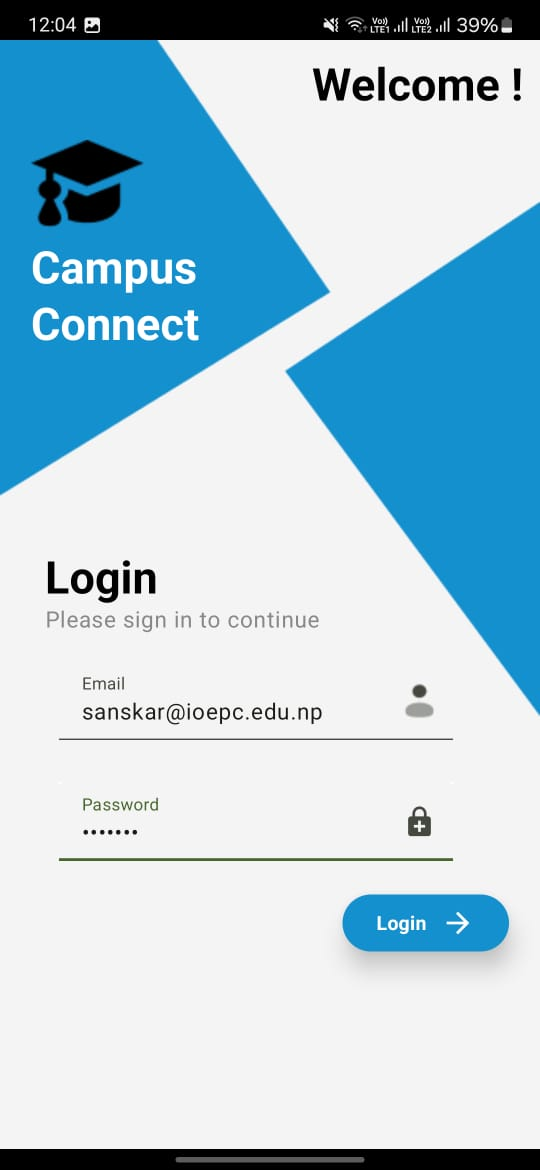
\includegraphics[width=0.5\textwidth]{Graphics/output/login_page.jpg}
    \caption{Login Page for Campus Connect}
    \label{fig:login_page}
\end{figure}

\subsection{Teacher Application}

\begin{figure}[H]
    \centering
    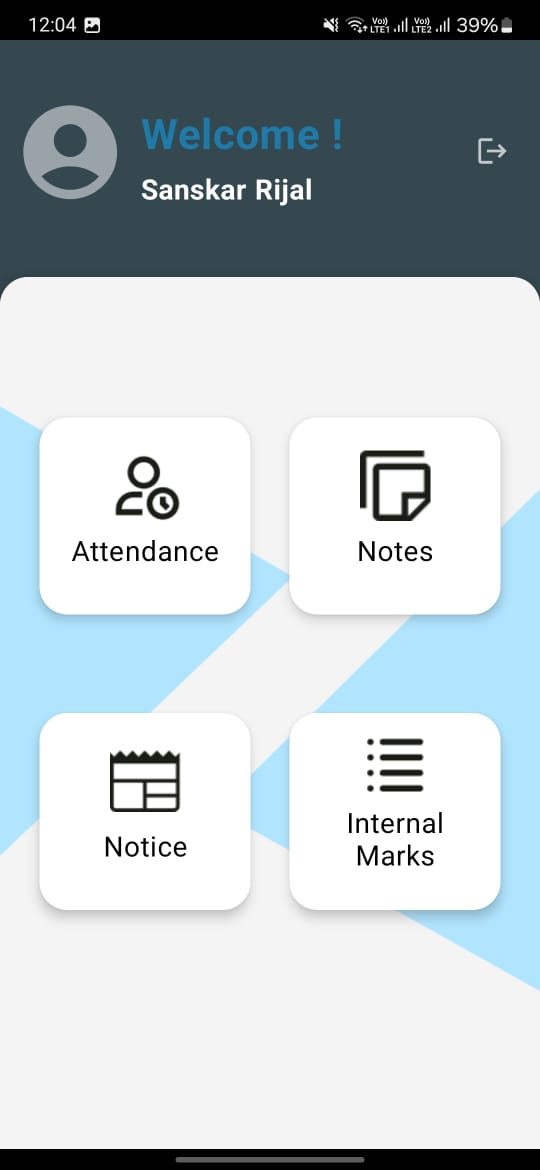
\includegraphics[width=0.5\textwidth]{Graphics/output/teacher_dashboard.jpg}
    \caption{Teacher Dashboard}
    \label{fig:teacher_dashboard}
\end{figure}

\begin{figure}[H]
    \centering
    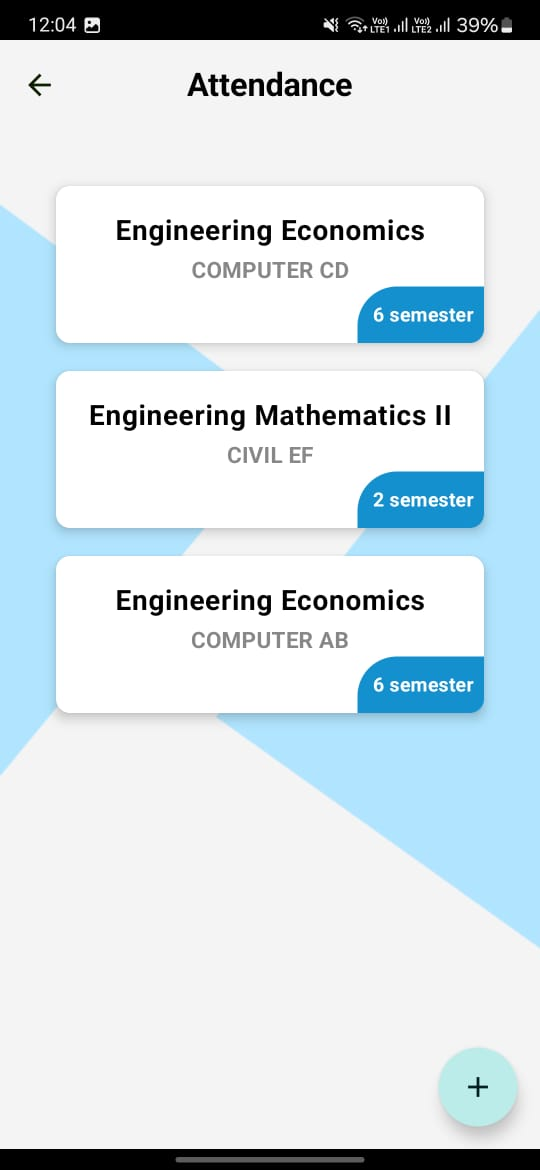
\includegraphics[width=0.5\textwidth]{Graphics/output/teacher_subjects.jpg}
    \caption{Subjects Added by Teacher}
    \label{fig:teacher_subjects}
\end{figure}

\begin{figure}[H]
    \centering
    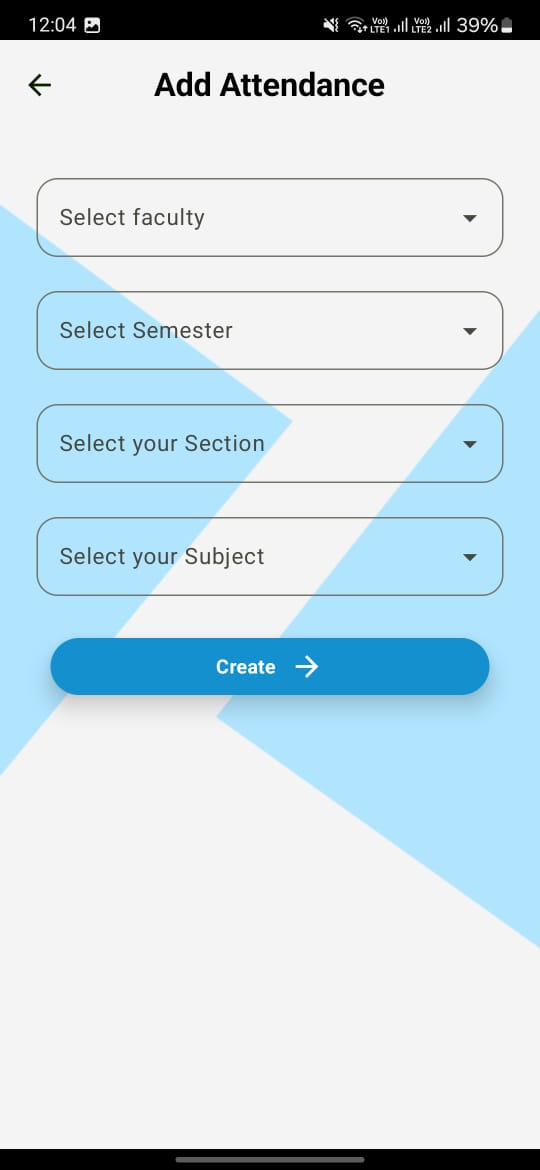
\includegraphics[width=0.5\textwidth]{Graphics/output/teacher_add_subject.jpg}
    \caption{Teacher Adding New Subject}
    \label{fig:teacher_add_subject}
\end{figure}

\begin{figure}[H]
    \centering
    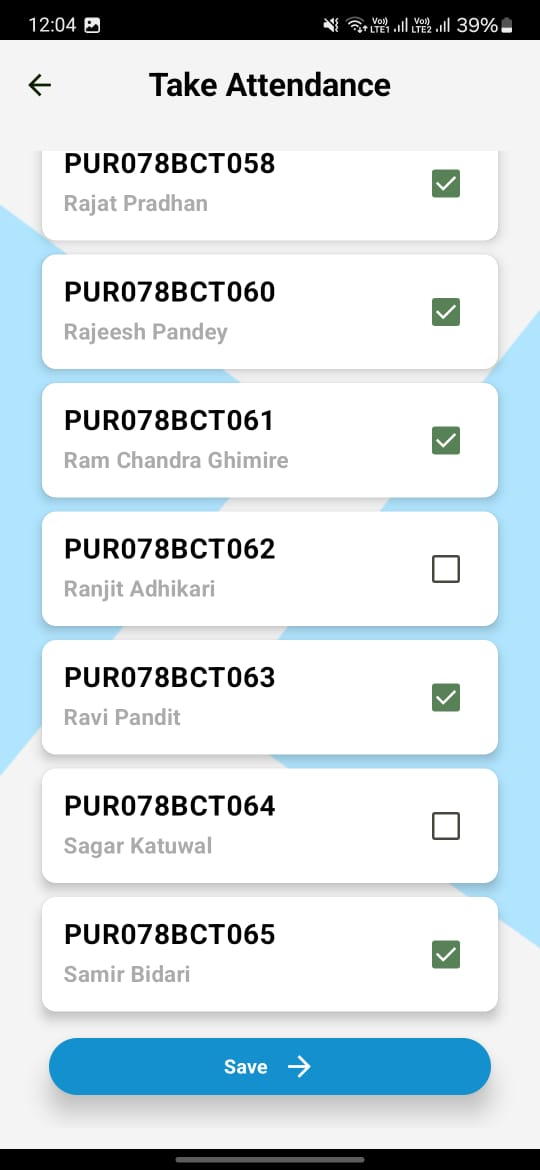
\includegraphics[width=0.5\textwidth]{Graphics/output/teacher_take_attendance.jpg}
    \caption{Teacher Taking Attendance}
    \label{fig:teacher_take_attendance}
\end{figure}

\begin{figure}[H]
    \centering
    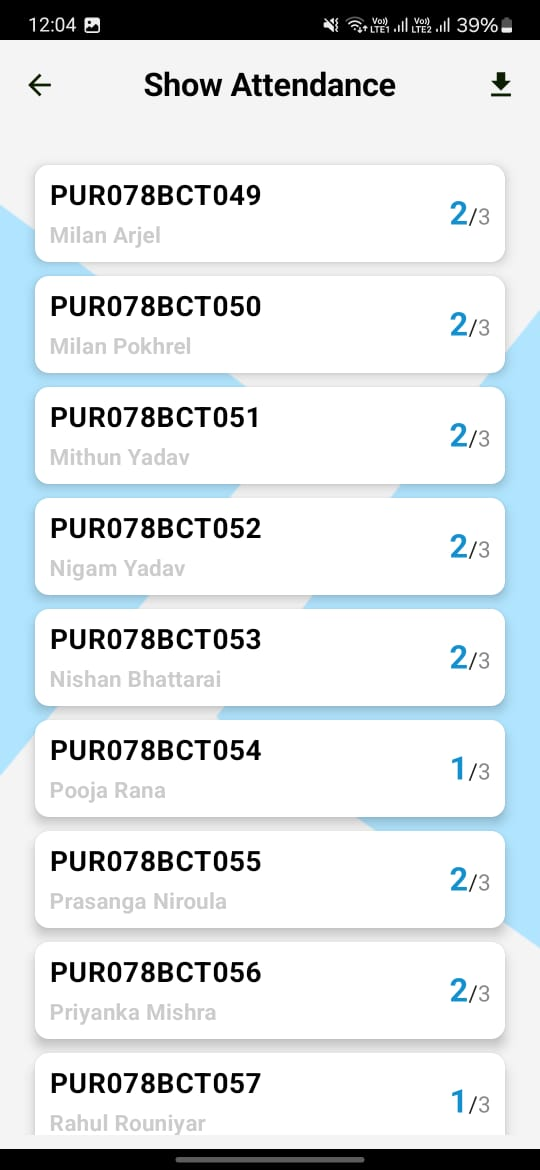
\includegraphics[width=0.5\textwidth]{Graphics/output/teacher_show_attendance.jpg}
    \caption{Teacher Viewing Attendance Records}
    \label{fig:teacher_show_attendance}
\end{figure}

\begin{figure}[H]
    \centering
    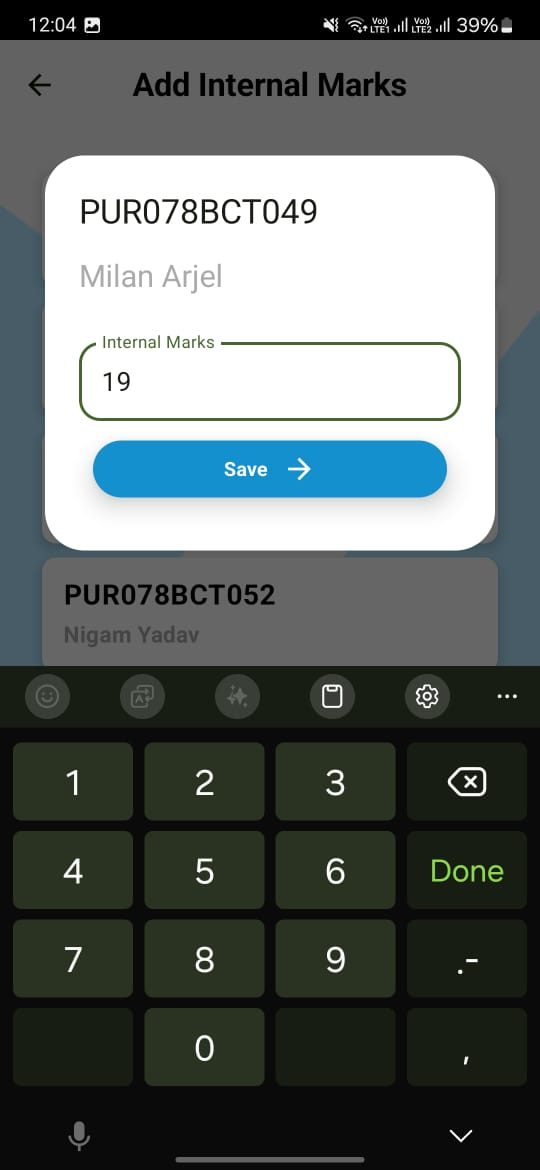
\includegraphics[width=0.5\textwidth]{Graphics/output/teacher_add_marks.jpg}
    \caption{Teacher Adding Internal Marks}
    \label{fig:teacher_add_marks}
\end{figure}

\begin{figure}[H]
    \centering
    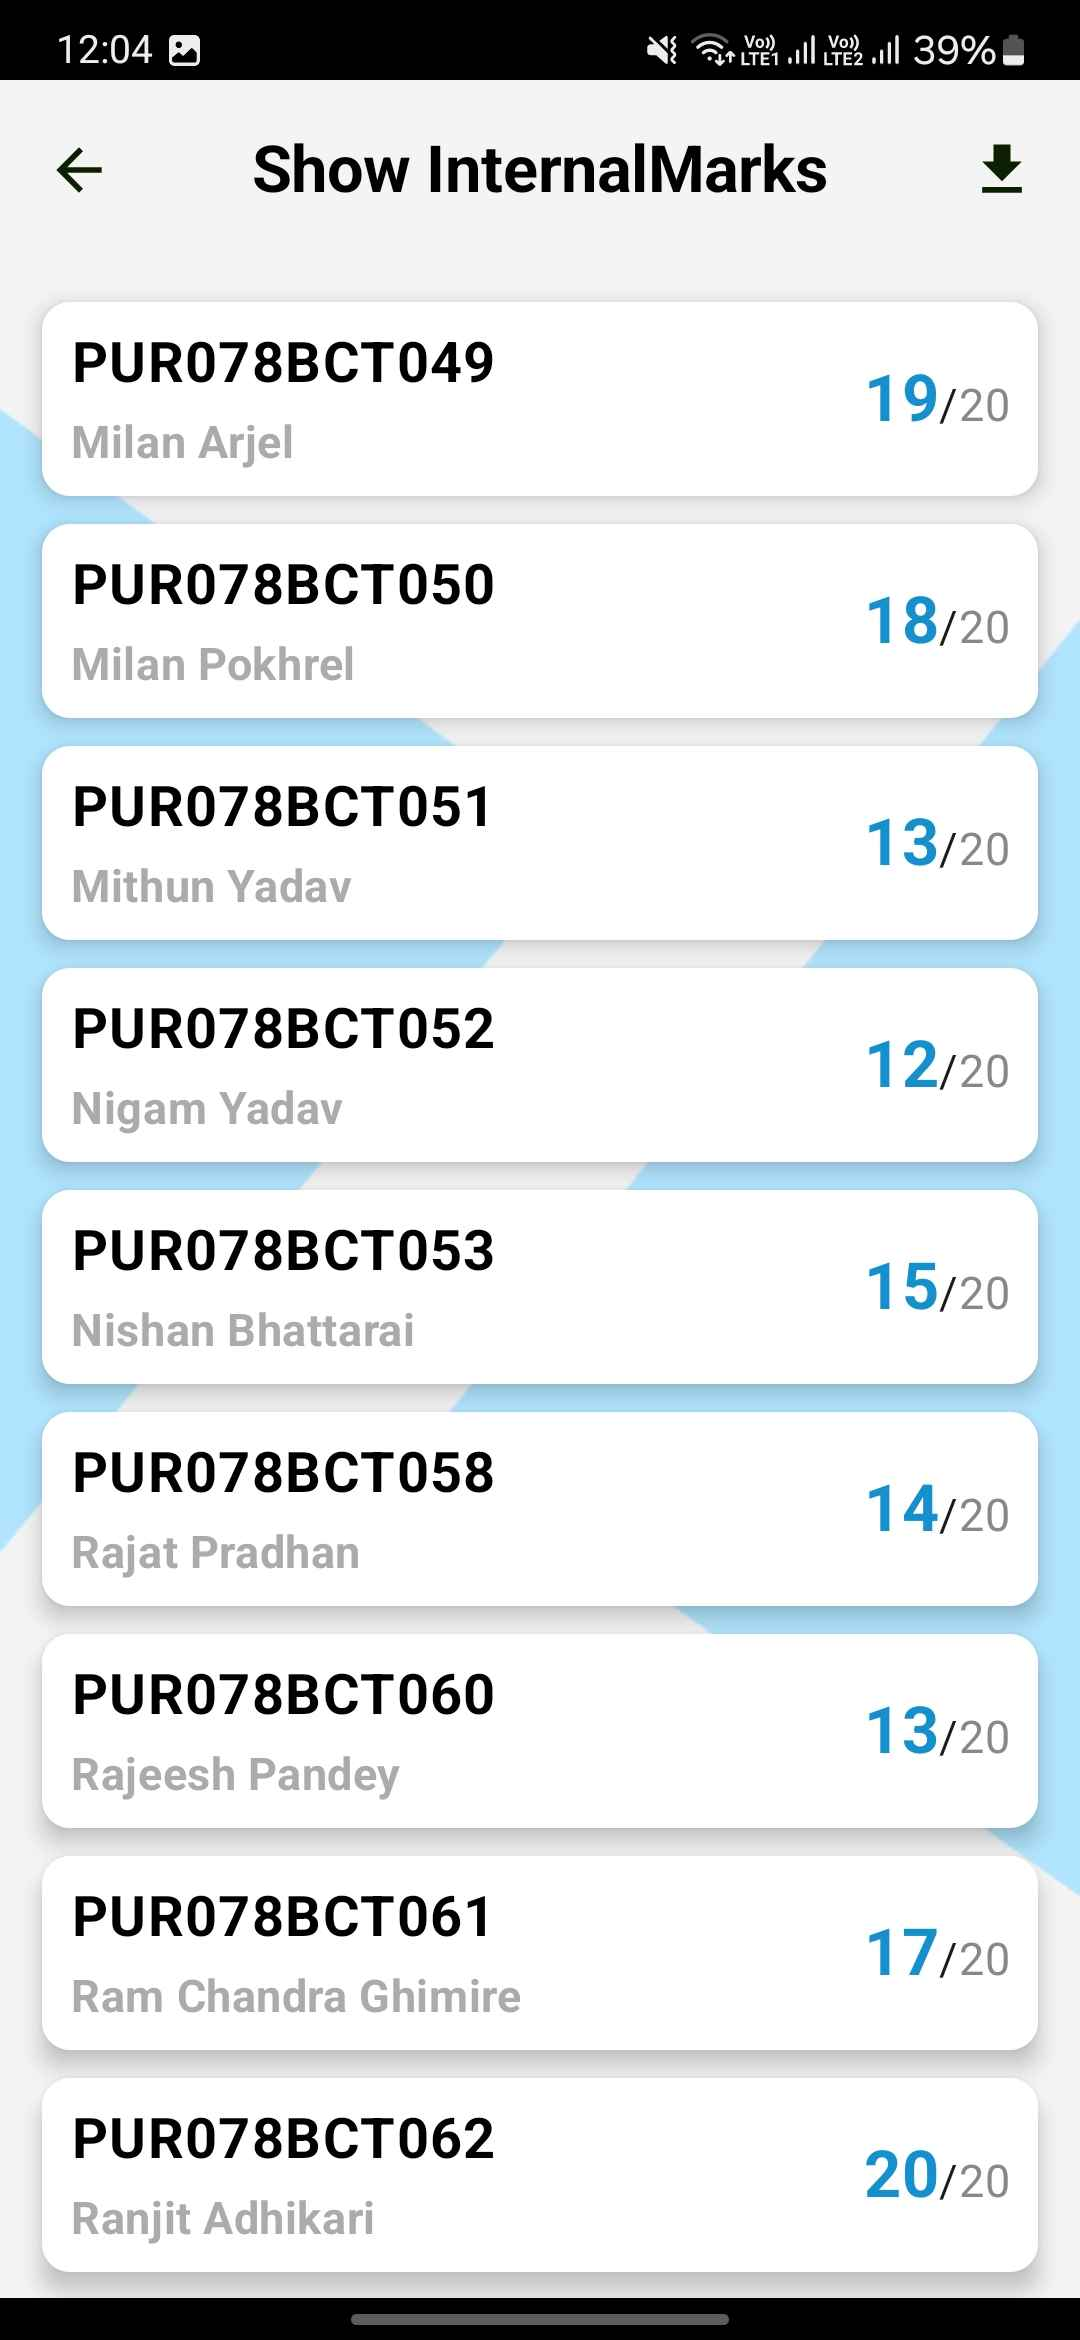
\includegraphics[width=0.5\textwidth]{Graphics/output/teacher_show_marks.jpg}
    \caption{Teacher Viewing Internal Marks}
    \label{fig:teacher_show_marks}
\end{figure}

\begin{figure}[H]
    \centering
    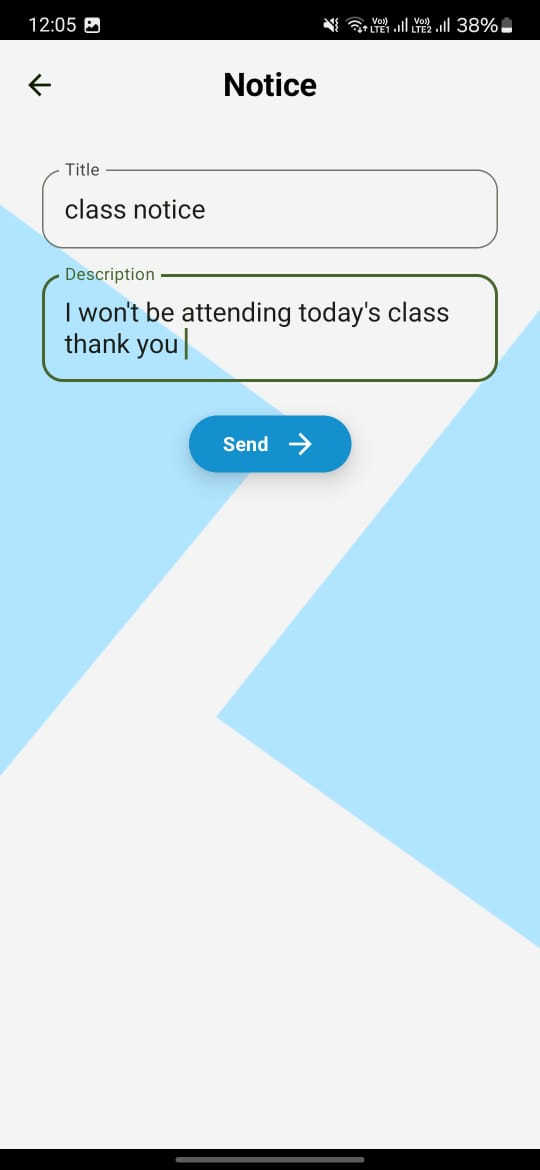
\includegraphics[width=0.5\textwidth]{Graphics/output/teacher_add_notice.jpg}
    \caption{Teacher Adding Notice}
    \label{fig:teacher_add_notice}
\end{figure}

\begin{figure}[H]
    \centering
    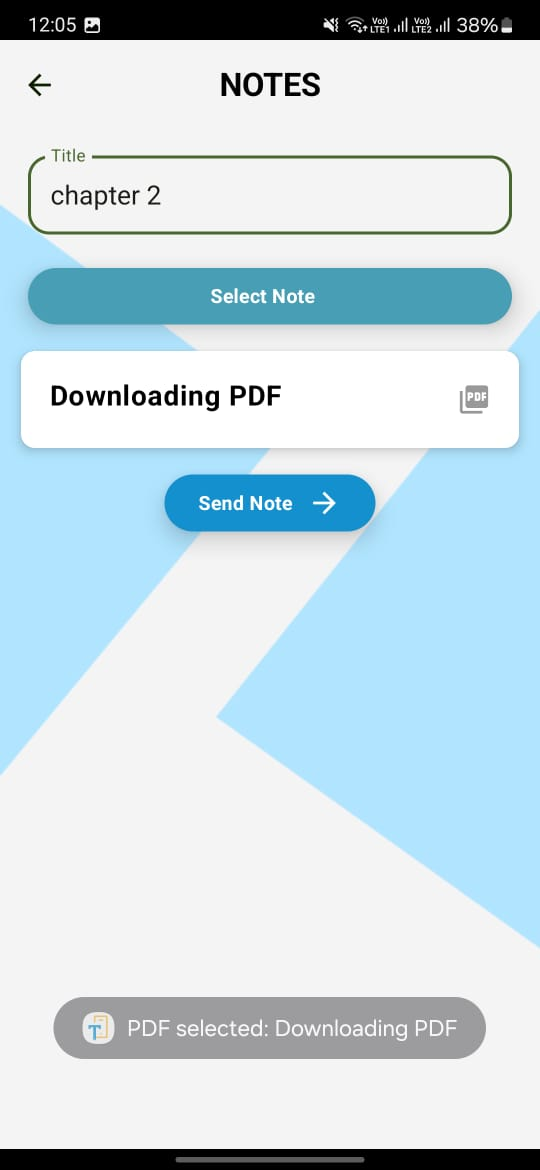
\includegraphics[width=0.5\textwidth]{Graphics/output/teacher_add_notes.jpg}
    \caption{Teacher Adding Notes}
    \label{fig:teacher_add_notes}
\end{figure}

\subsection{Student Application}

\begin{figure}[H]
    \centering
    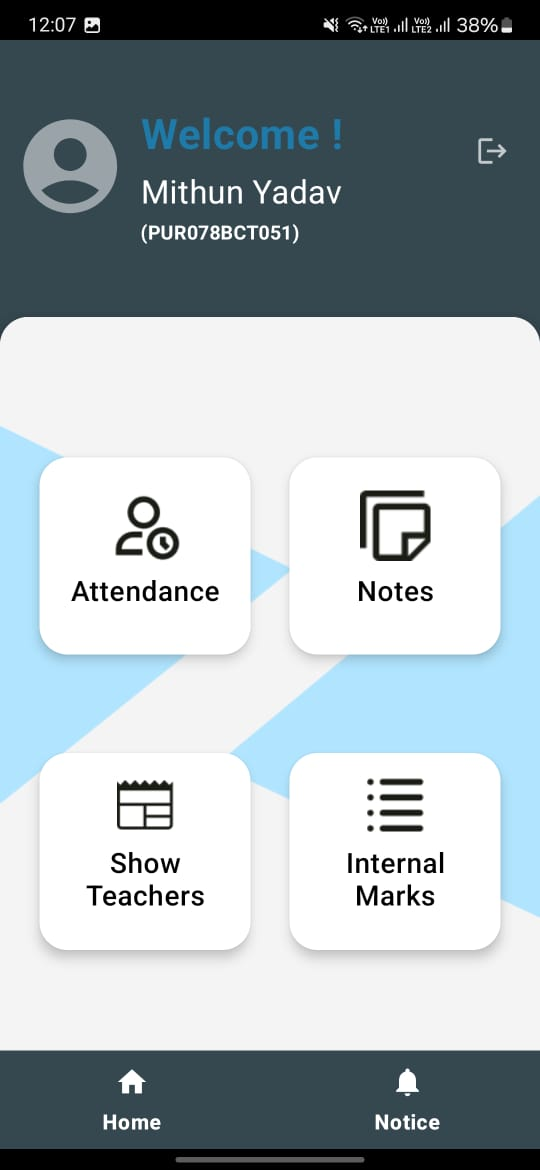
\includegraphics[width=0.5\textwidth]{Graphics/output/student_dashboard.jpg}
    \caption{Student Dashboard}
    \label{fig:student_dashboard}
\end{figure}

\begin{figure}[H]
    \centering
    
\includegraphics[width=0.5\textwidth]{Graphics/output/student_attendance.jpg}
    \caption{Student Viewing Attendance}
    \label{fig:student_attendance}
\end{figure}

\begin{figure}[H]
    \centering
    
\includegraphics[width=0.5\textwidth]{Graphics/output/student_marks.jpg}
    \caption{Student Viewing Internal Marks}
    \label{fig:student_marks}
\end{figure}

\begin{figure}[H]
    \centering
    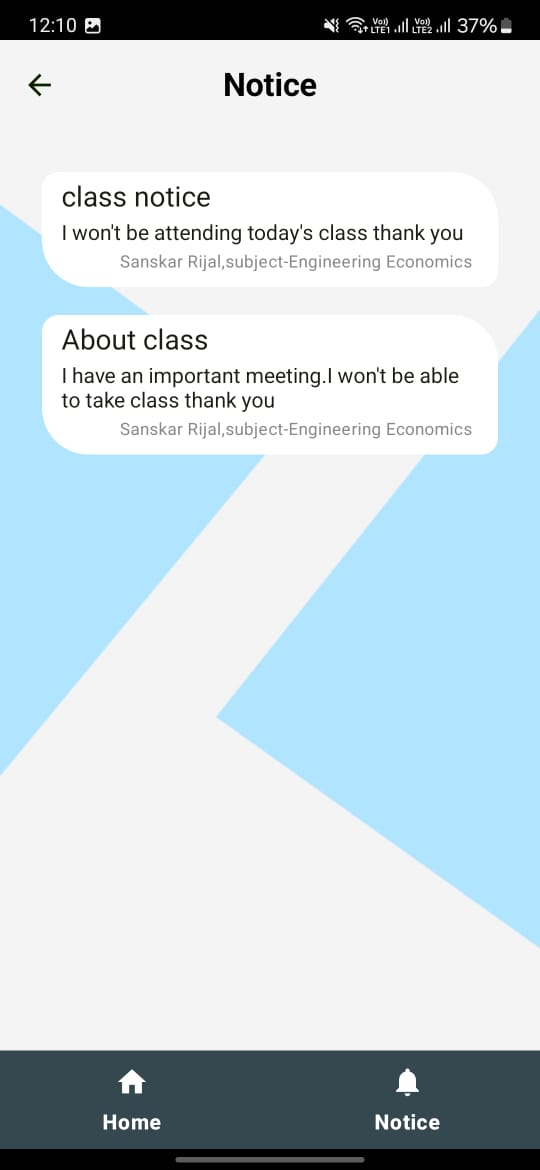
\includegraphics[width=0.5\textwidth]{Graphics/output/student_notices.jpg}
    \caption{Student Viewing Notices}
    \label{fig:student_notices}
\end{figure}

\begin{figure}[H]
    \centering
    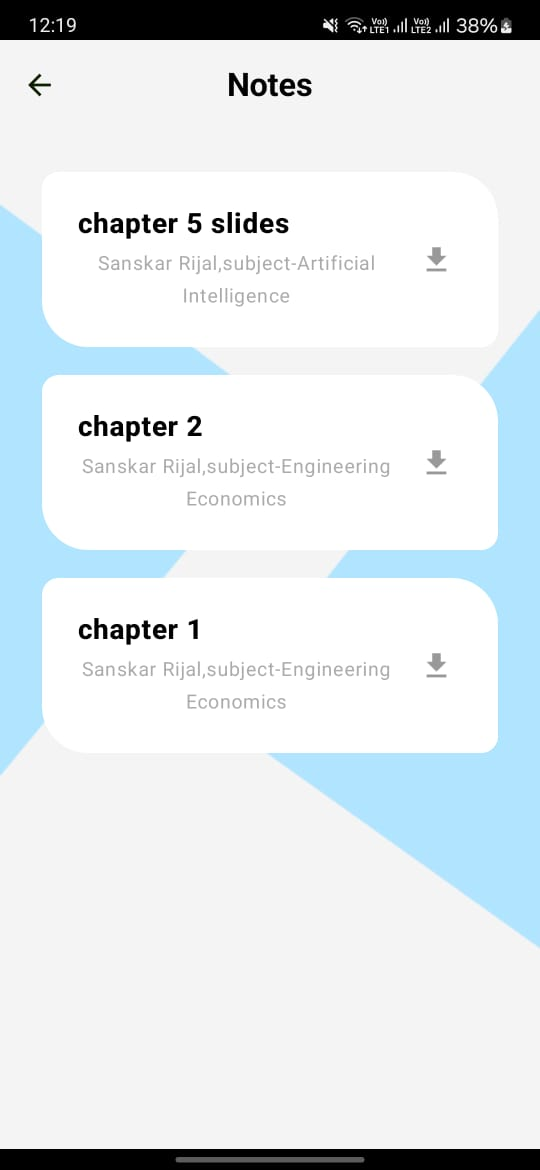
\includegraphics[width=0.5\textwidth]{Graphics/output/student_notes.jpg}
    \caption{Student Accessing Notes}
    \label{fig:student_notes}
\end{figure}

\begin{figure}[H]
    \centering
    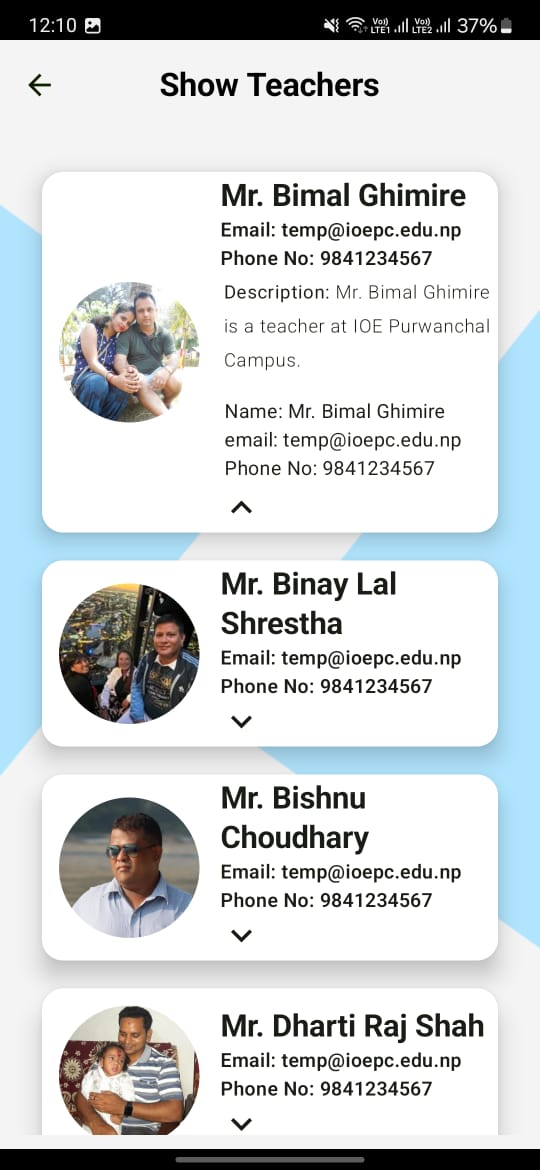
\includegraphics[width=0.5\textwidth]{Graphics/output/student_view_teachers.jpg}
    \caption{Student Viewing Teacher Information}
    \label{fig:student_view_teachers}
\end{figure}

\section{Summary}
The screenshots above demonstrate the key features of the Campus Connect application, providing an efficient way for students to access academic information and for teachers to manage course content, attendance, and assessments.